%--------------------------------------------------------------------------------%
\section{CASO DE USO}\label{sec:caso_de_uso}

O principal objetivo da ferramenta computacional é iterar modelos utilizando alguma lógica pré-definida por algum algoritmo disponível. Através dos comandos descritos na Seção~\ref{sec:console} é possível que estes modelos sejam criados, alterados, iterados e, opcionalmente, visualizados. Com isto o principal fluxo de uso foi disponibilizado.

\begin{figure}[!htbp]
	\centering
	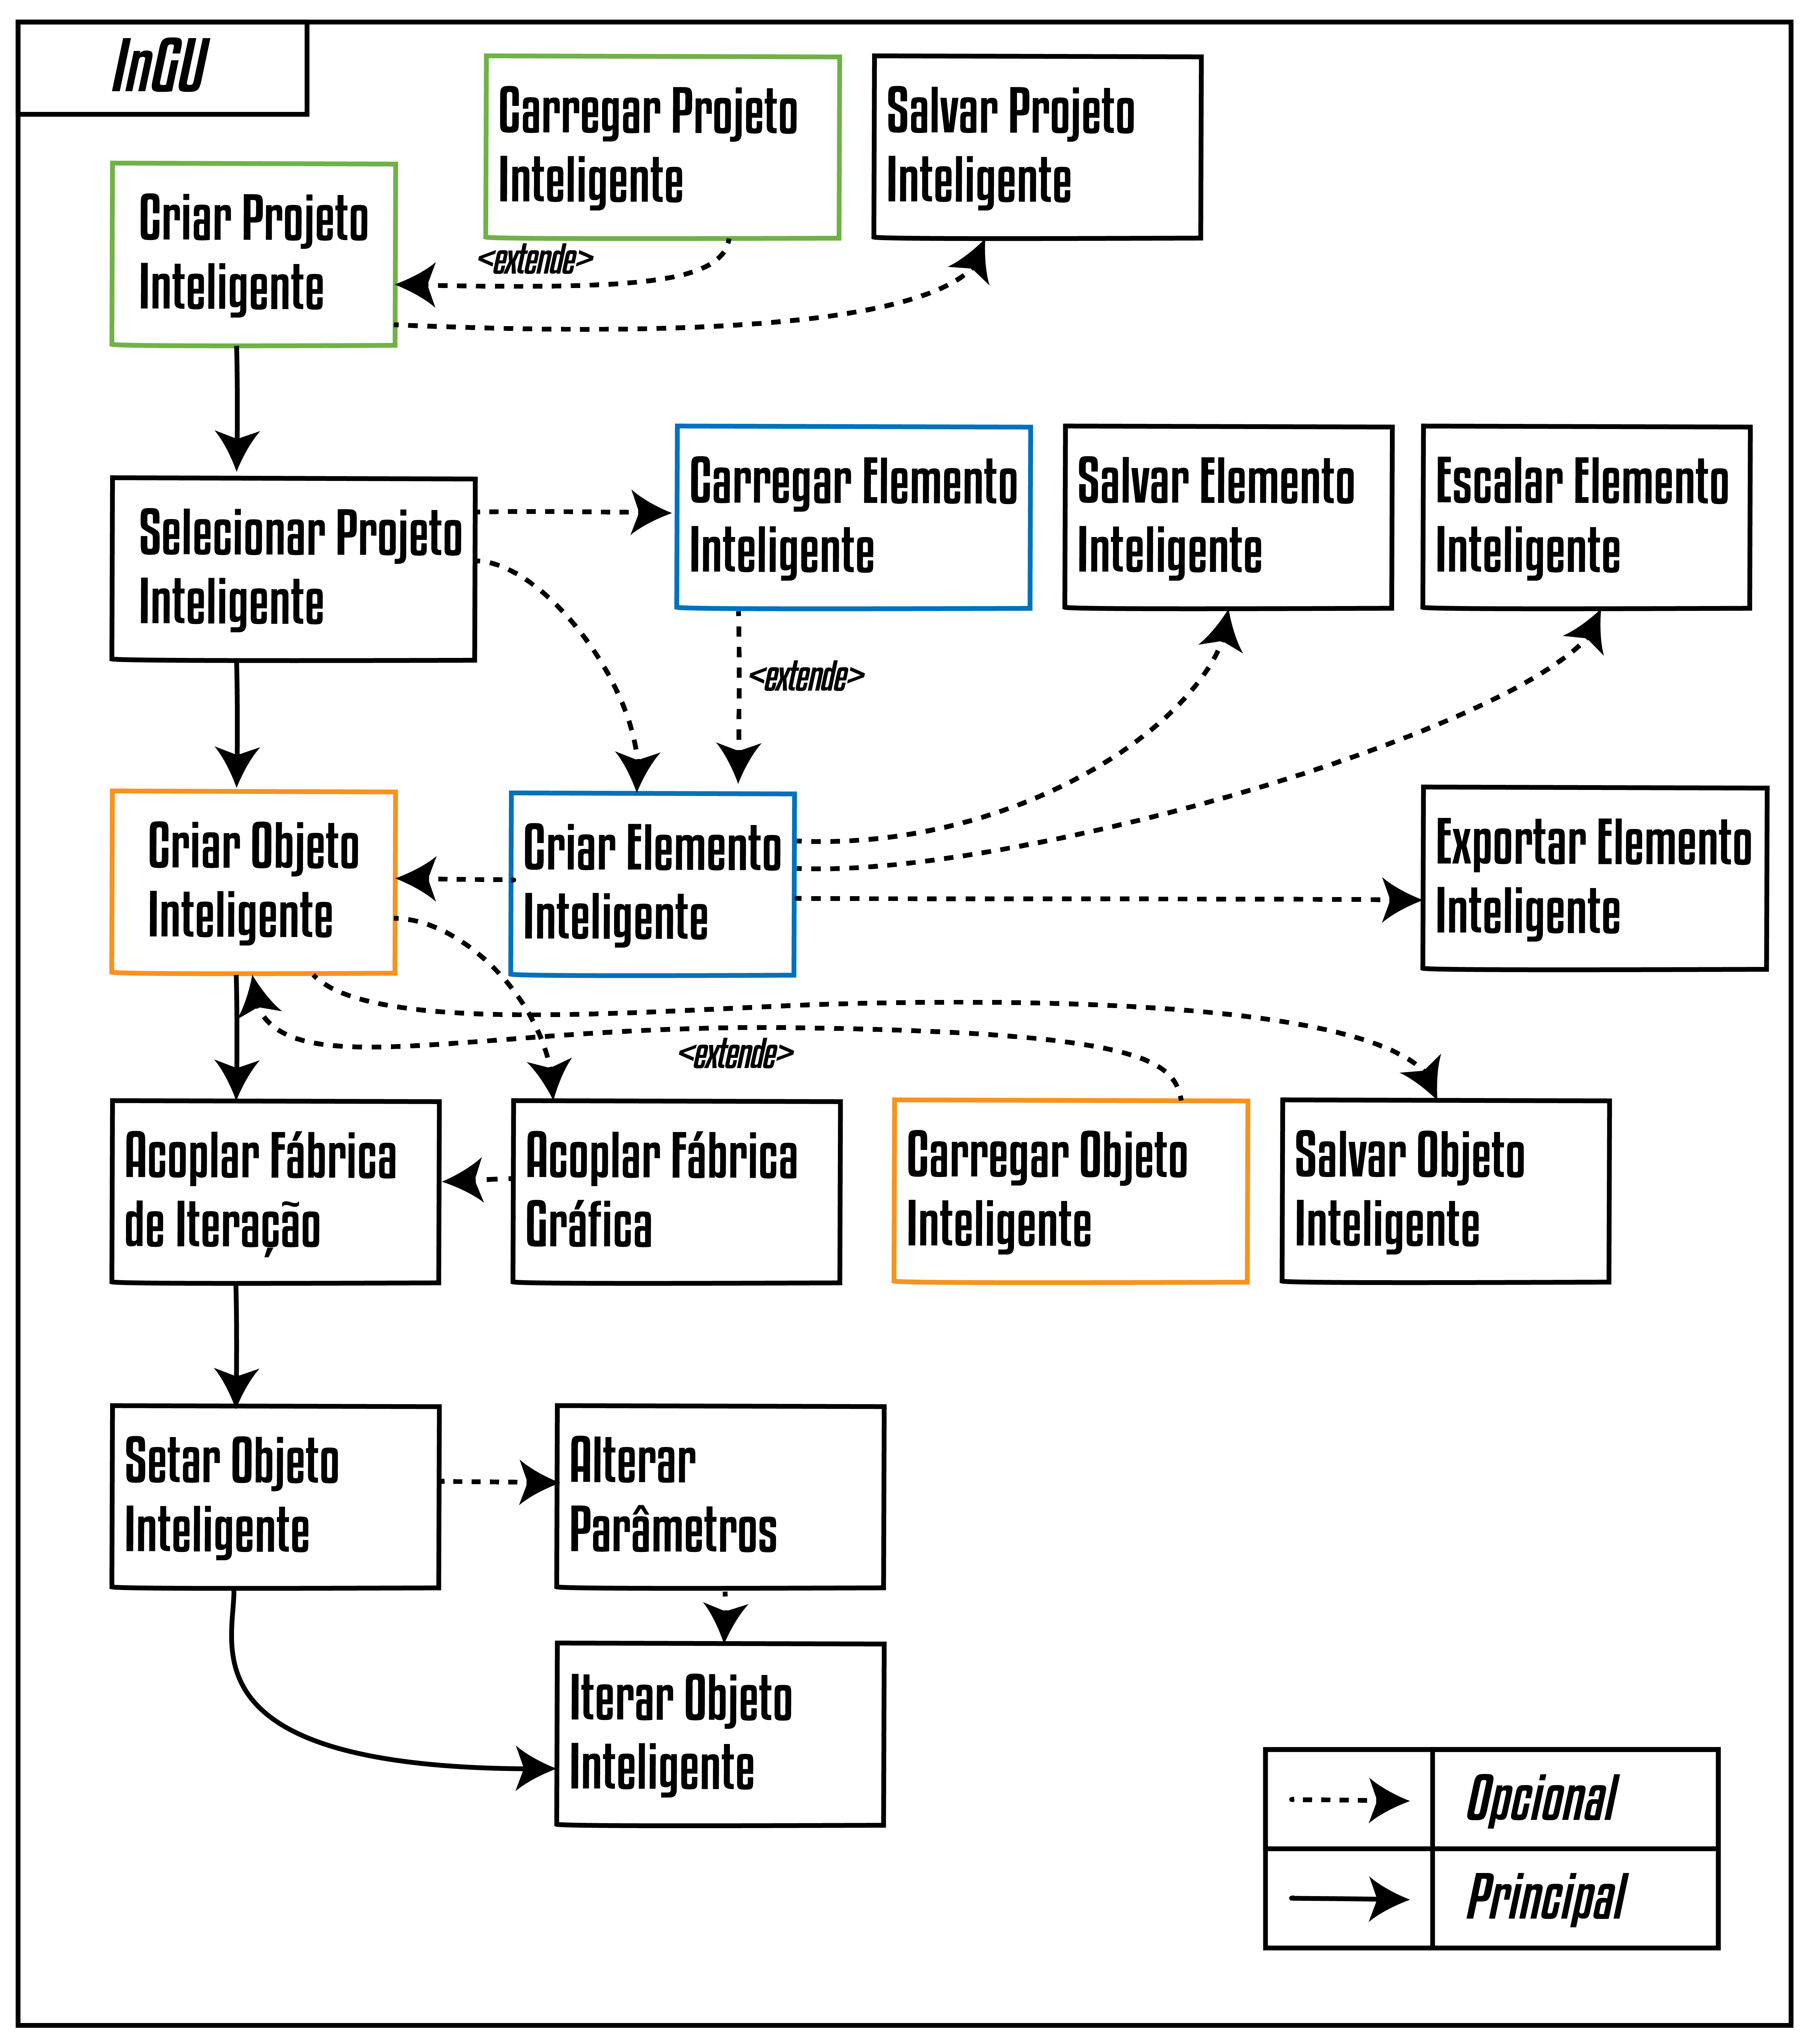
\includegraphics[width=\linewidth]{Figures/CasoDeUso@16x.png}
	\caption{Fluxograma do ambiente computacional InGU, em azul as atividades de criação de elementos inteligentes, em verde as atividades de criação de projetos inteligentes e em laranja as atividades de criação de objetos inteligentes.}
	\label{fig:caso_uso}
\end{figure}

A Figura~\ref{fig:caso_uso} demonstra a principal sequência de atividades executadas para se iterar um objeto inteligente. Como descrito na Seção~\ref{sec:estrutura}, um objeto inteligente recém-criado não pode ser iterado, ele precisa antes ser corretamente configurado. Com este modelo é possível observar a sequência de passos necessárias para se iterar um obejto inteligente.

Primeiramente, é necessário criar um projeto inteligente e selecioná-lo. Cada atividade representada no fluxograma é executada por um comando correspondente, o mesmo fluxo pode ser observado no Anexo~\ref{annex2}. As primeiras linhas de comando representadas neste arquivo de comandos são de criação de projetos.

Ao criar um objeto inteligente, seus elemento inteligentes são juntamente criados, ambas estas funcionalidades estão disponíveis ao usuário uma vez que ele tenha selecionado um projeto. É possível ainda que se cria um objeto inteligente à partir de um elemento inteligente, desta forma é garantida também a igualdade inicial entre os modelos.

Com um objeto criado corretamente é possível adicionar à ele uma fábrica de iteração e uma gráfica. Ao acoplar a fábrica de iteração o método iterativo é liberado, bem como a possibilidade de alterar os parâmetros do objeto inteligente.

Foi adicionada também a possibilidade de se exportar elementos inteligentes, para o caso de alguns elementos inteligentes como \textit{WiseGraphic} isso siginifca a exportação de imagem no formato \textbf{P}ortable \textbf{N}etwork \textbf{G}raphics, ou \textit{png}, com seu comando representado na linha $7$ do Anexo~\ref{annex2}.

Como mencionado anteriormente, a mesma estrutura foi utilizada na construção do ambiente computacional composto por elementos gráficos \textit{IGU}. Desta forma o principal fluxo de uso da interface gráfica foi desenvolvido.

\begin{figure}[!htbp]
	\centering
	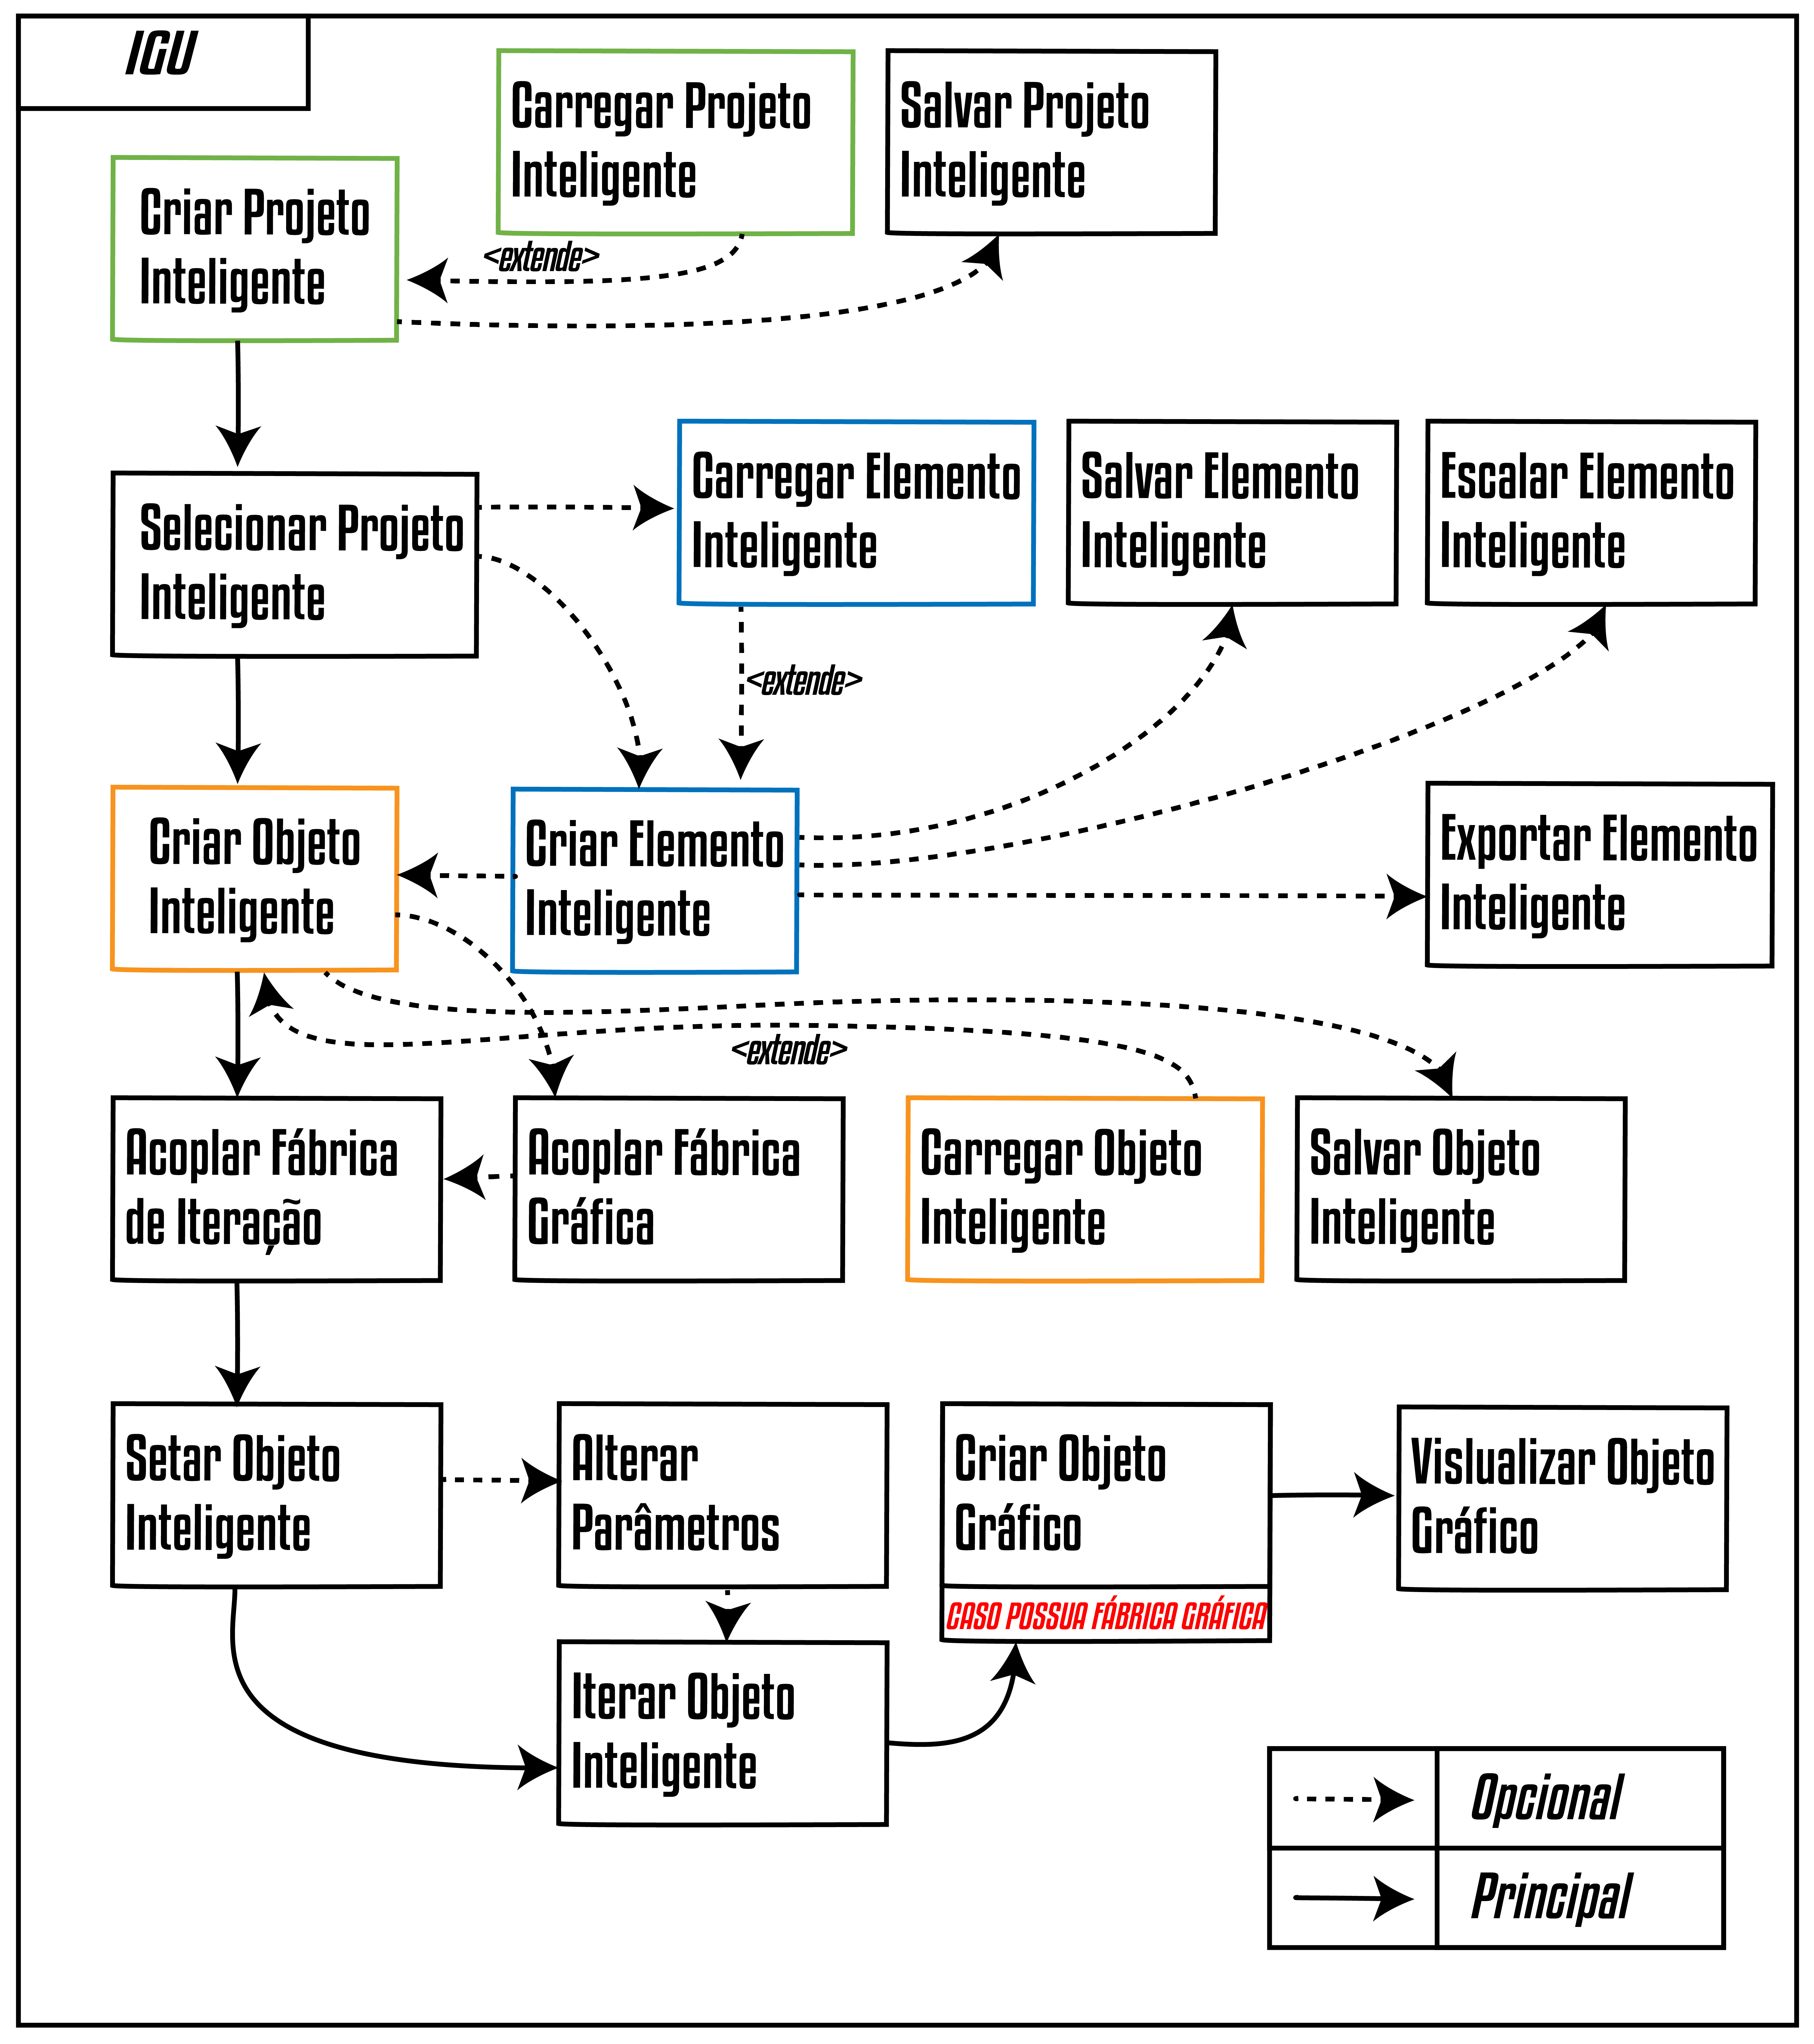
\includegraphics[width=\linewidth]{Figures/CasoDeUso2@16x.png}
	\caption{Fluxo de caso de uso do ambiente computacional IGU.}
	\label{fig:caso_uso2}
\end{figure}

Finalmente, o funcionamento apresentado pela Figura~\ref{fig:caso_uso2} difere do apresentado na Figura~\ref{fig:caso_uso} apenas na visualização dos objetos gráficos disponibilizada pelos elementos gráficos. Isto garante que ambos os ambientes computacionais sejam alterados em uma eventual atualização de código e que tenham funcionamento idêntico.

%--------------------------------------------------------------------------------%
\section{JANELA PRINCIPAL}\label{sec:janela}

O ambiente com interface gráfica foi nomeado de \textbf{I}terador \textbf{G}ráfico \textbf{U}niversal, que também está presente como parte de um projeto \textit{Qt}/\textit{C++}. Diferentemente dos outro ambiente, este possui elementos gráficos. O principal elemento gráfico disponibilizado pela interface gráfico é a janela principal, que é um objeto do tipo \textit{QMainWindow}. Estes objetos são disponibilizados pela biblioteca \textit{Qt} e permitem que um projeto \textit{C++} possua uma interface gráfica utilizando diretivas OpenGL e GLUT (The OpenGL Utility Kit).

Ao abrir o ambiente computacional a tela principal com seus elementos gráficos é exibida.

\begin{figure}[!htbp]
	\centering
	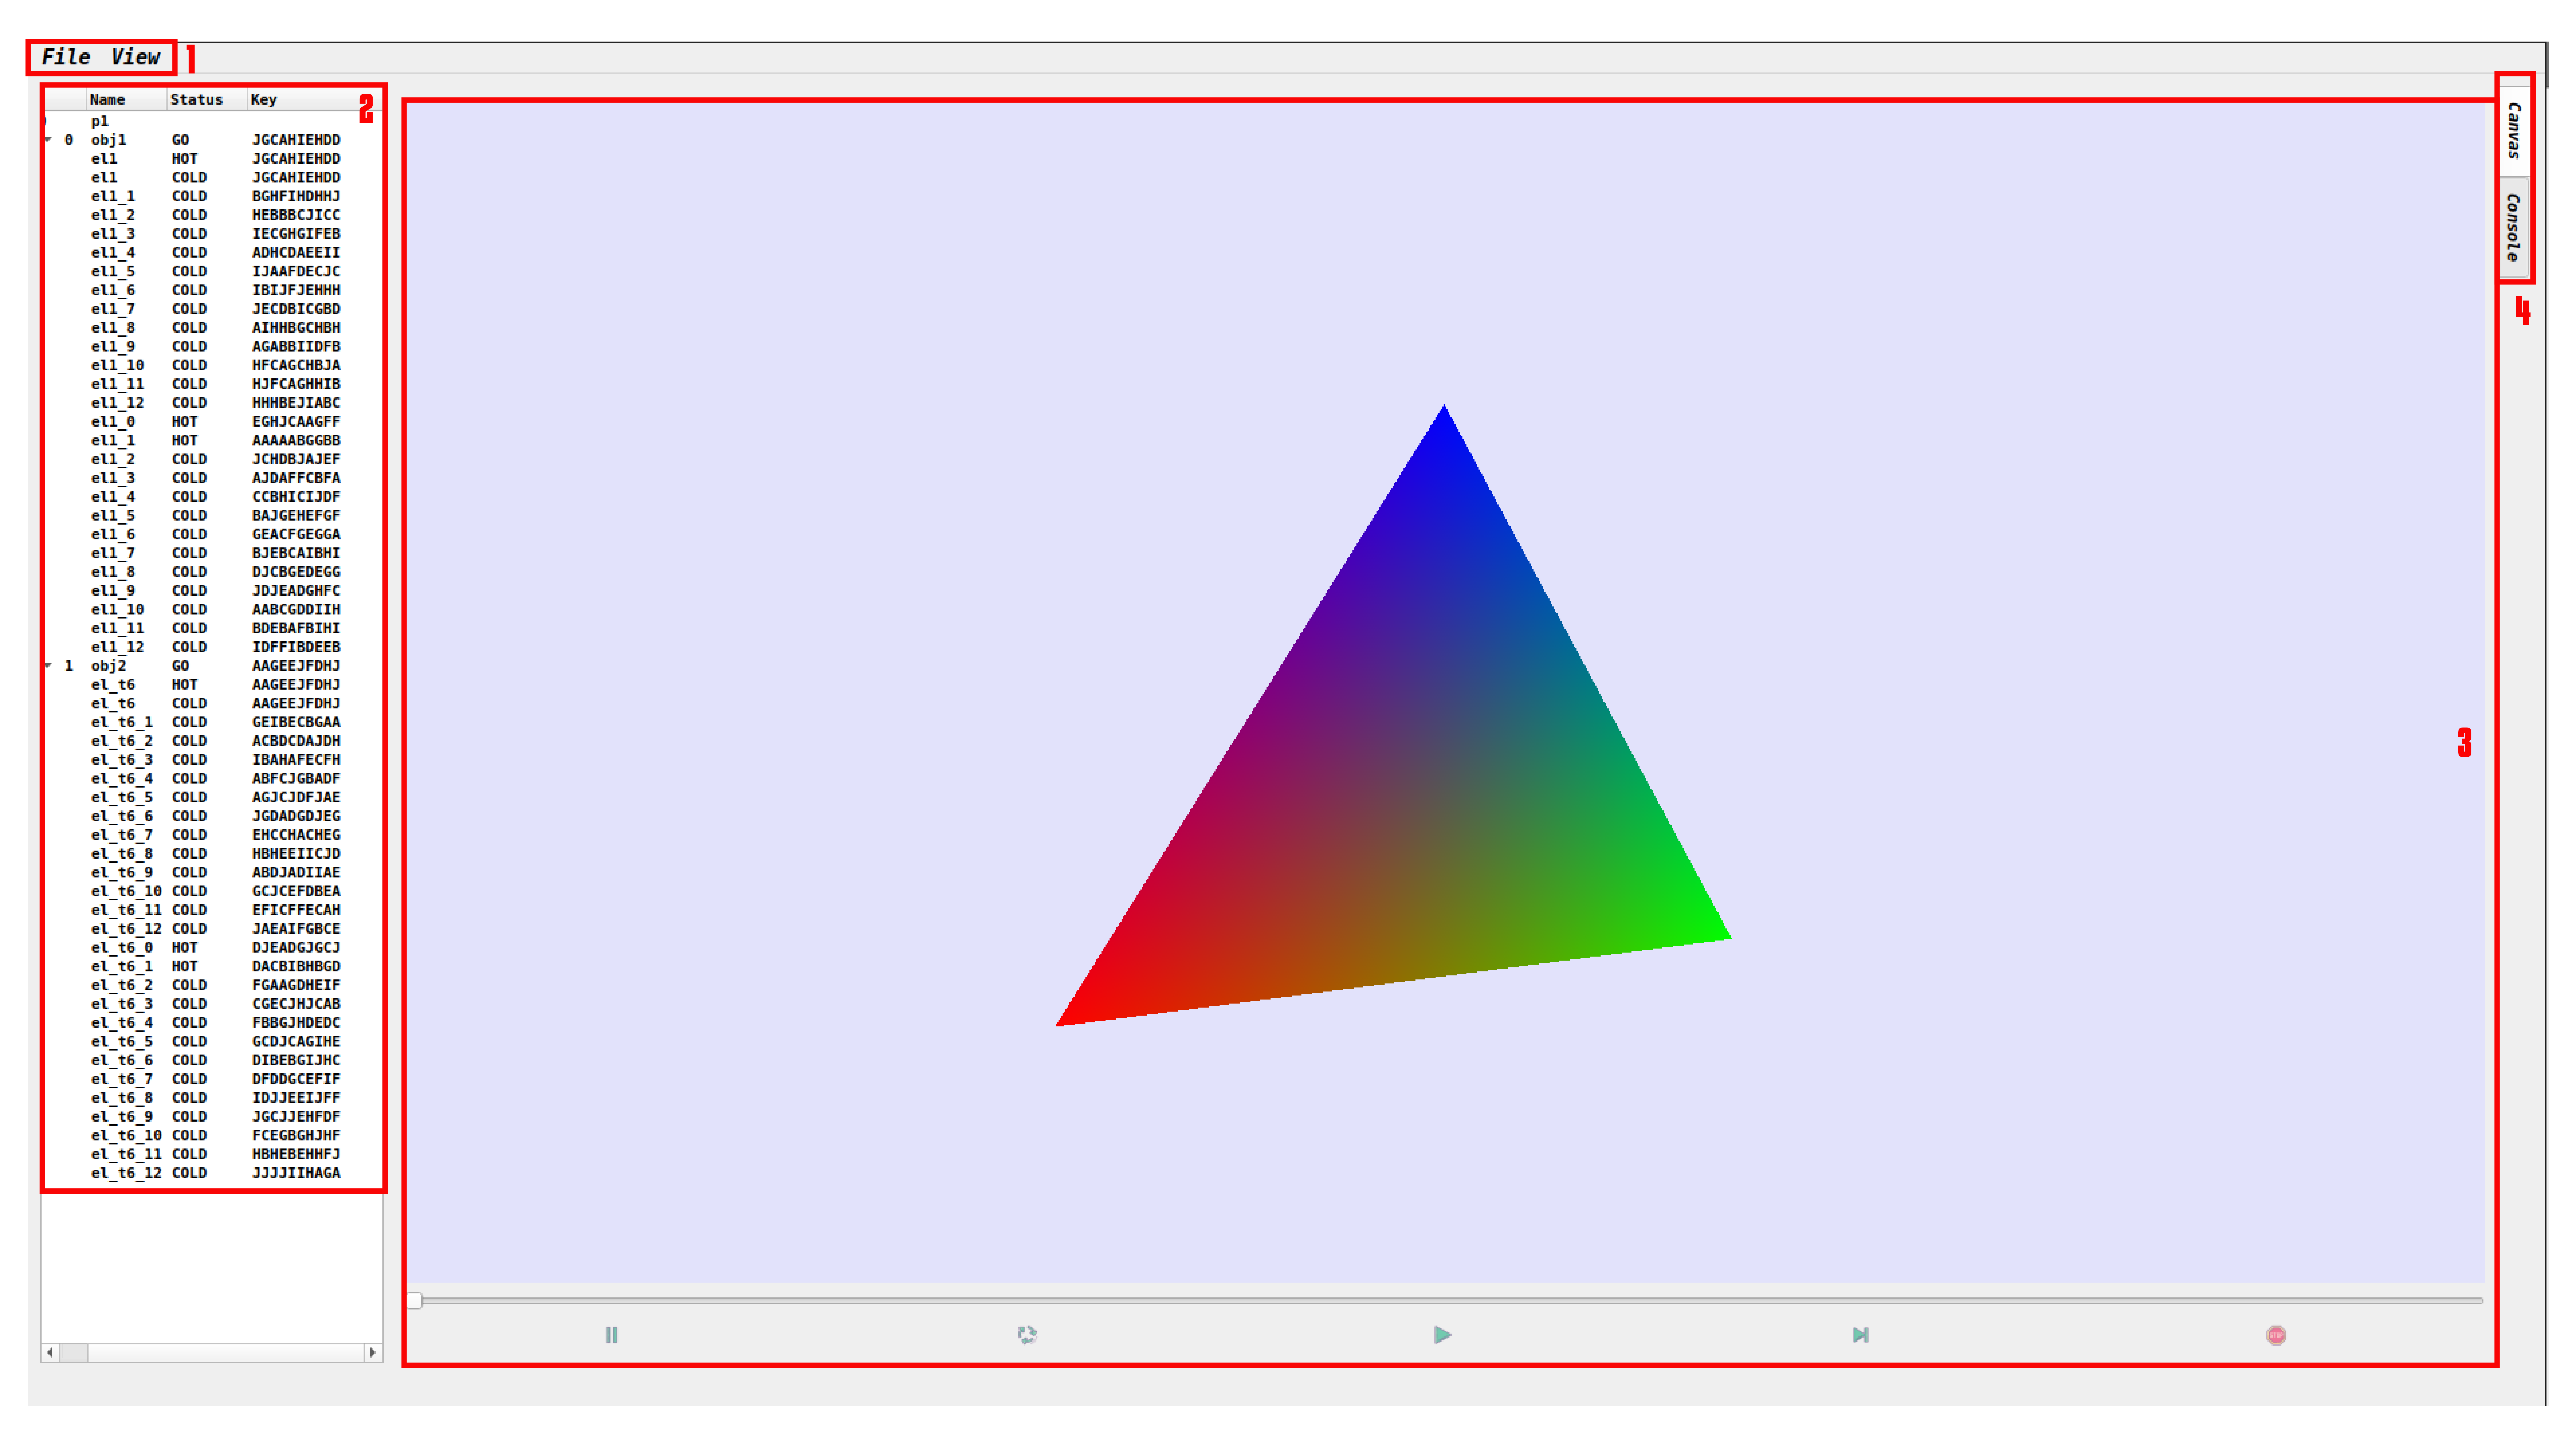
\includegraphics[width=\linewidth]{Figures/IGU_001a.png}
	\caption{Janela principal ambiente computacional IGU. Da esquerda para a direita: 1. Menu principal do programa; 2. Árvore de projetos e seus elementos; 3. Área de trabalho, no caso mostrando OpenGl \textit{Canvas}; 4. Seleção de abas}
	\label{fig:UI}
\end{figure}

A Figura~\ref{fig:UI} demonstra o comportamento inicial da ferramenta computacional. Ao ser aberta o ambiente de trabalho é recuperado, projetos, objetos e elementos são recuperados de um arquivo contido na mesma parta da ferramenta computacional. Este arquivo é salvo toda vez que a ferramenta computacional é encerrada com projetos inteligentes ainda no ambiente. Ainda nesta figura estão representados os principais grupos de elementos gráficos.

As próximas seções discorrem sobre cada grupo de elemento gráfico presente na janela principal da ferramenta computacional e seu funcionamento.

%--------------------------------------------------------------------------------%
\subsection{MENU}\label{sec:menu}

O primeiro grupo são os elementos que compões o menu principal da aplicação. Cada opção do menu é representada por um uma linha de texto, ao selecionar a linha uma ação é executada:

\begin{figure}[!htbp]
	\centering
	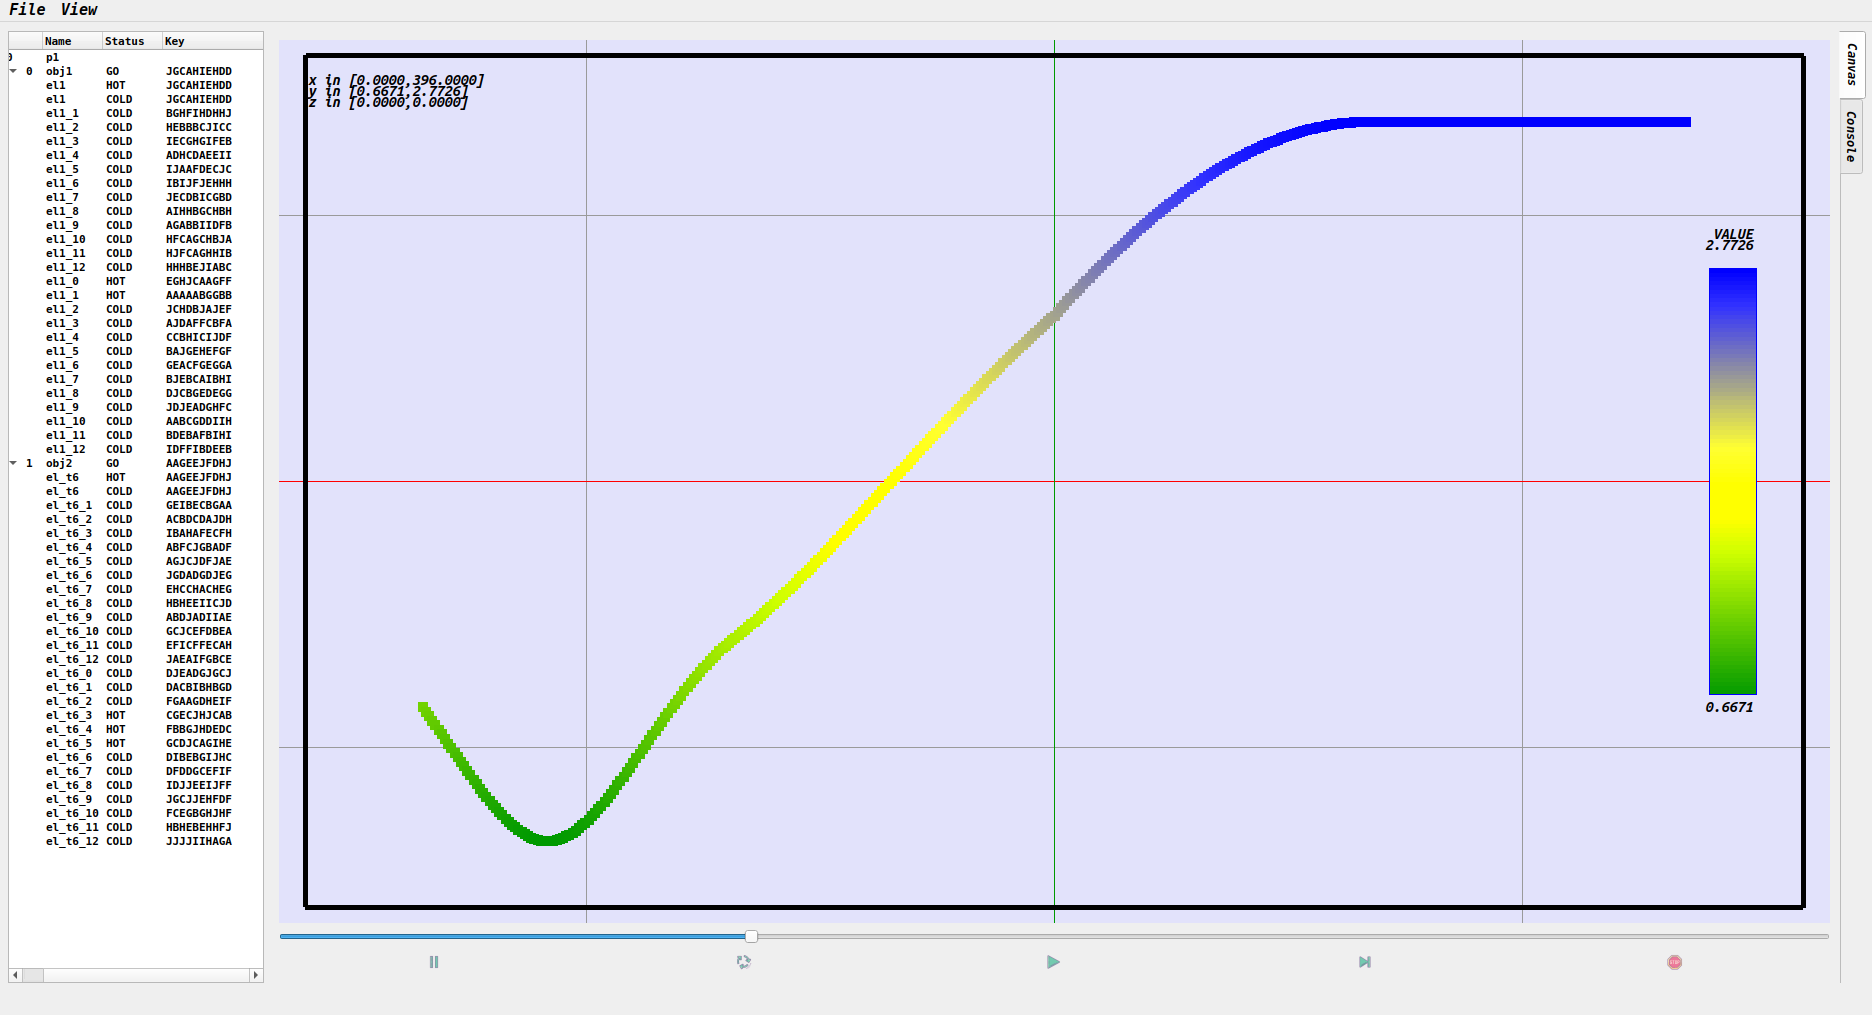
\includegraphics[scale=1]{Figures/IGU_016.png}
	\caption{Opções do menu principal da ferramenta computacional \textit{IGU}}
	\label{fig:menu}
\end{figure}


\begin{itemize}
	\item \textbf{Exit}: Fecha o ambiente computacional.
	\item \textbf{Jobs}: Abre a Janela que exibe os trabalhos inteligentes criados.
	\item \textbf{Open Canvas}: Abre uma nova janela contendo um novo elemento gráfico OpenGL \textit{Canvas}.
\end{itemize}

Ao abrir um novo elemento gráfico \textit{Canvas}, uma nova listagem é exibida ao executar o comando de listar canvas. Isso possibilita que mais de um objeto seja exibido ao mesmo tempo em janelas distintas.

%--------------------------------------------------------------------------------%
\subsection{ABAS \& ÁREA DE TRABALHO}\label{sec:abas}

As abas da janela principal selecionam o elemento de interface gráfica que será exibido na área de trabalho da aplicação.

\begin{figure}[!htbp]
	\centering
	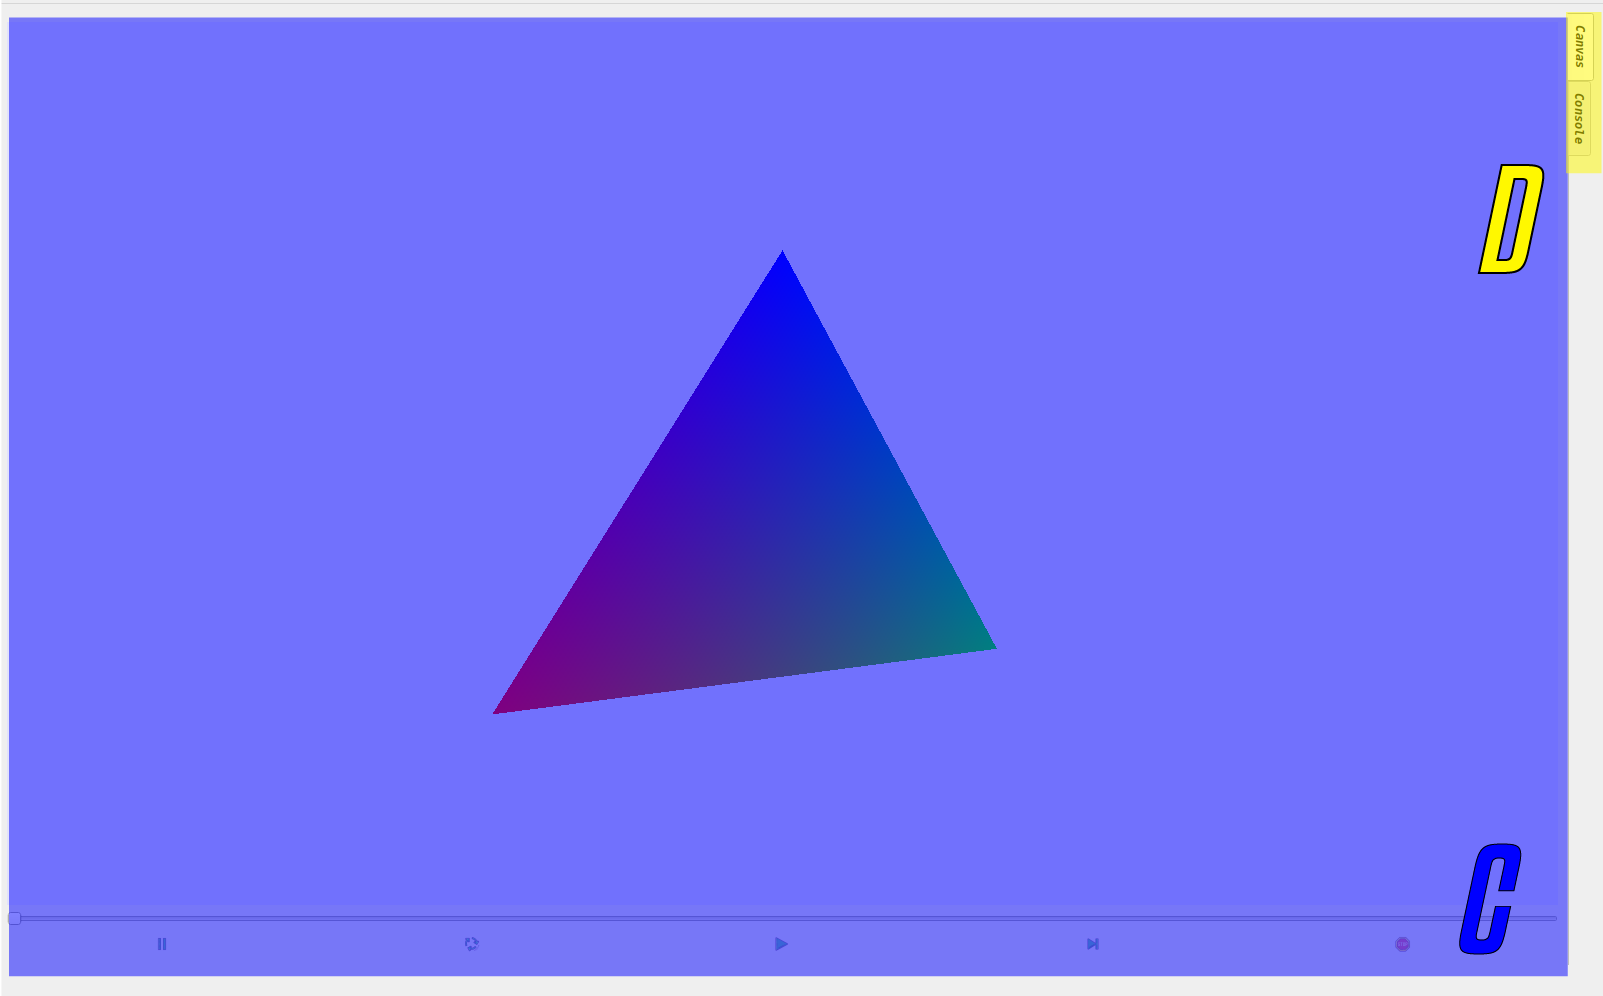
\includegraphics[width=\linewidth]{Figures/IGU_001a_34.png}
	\caption{Opções do menu principal da ferramenta computacional \textit{IGU}}
	\label{fig:abas}
\end{figure}

Ao selecionar uma das abas, os elementos de interface de usuário da área de trabalho são trocados. Estes elementos são objetos do tipo \textit{QWidget}, estes objetos que são divididos em dois ambientes, o \textit{Canvas} e o \textit{Console}. 

Ao selecionar a opção do \textit{Console} um ambiente similar ao disponibilizado pelo ambiente \textit{InGU} é disponibilizado. Utilizando um elemento de exibição textual longa, uma linha de texto como entrada e um botão, os mesmo comandos disponibilizados na Seção~\ref{sec:console} são acessados por estes elementos gráficos. Para executar uma linha de comando basta inserir-la no elemento gráfico e pressionar o botão ou a tecla \textit{Enter}, a resposta será acoplada ao elemento de exibição textual longa.

\begin{figure}
	\centering
	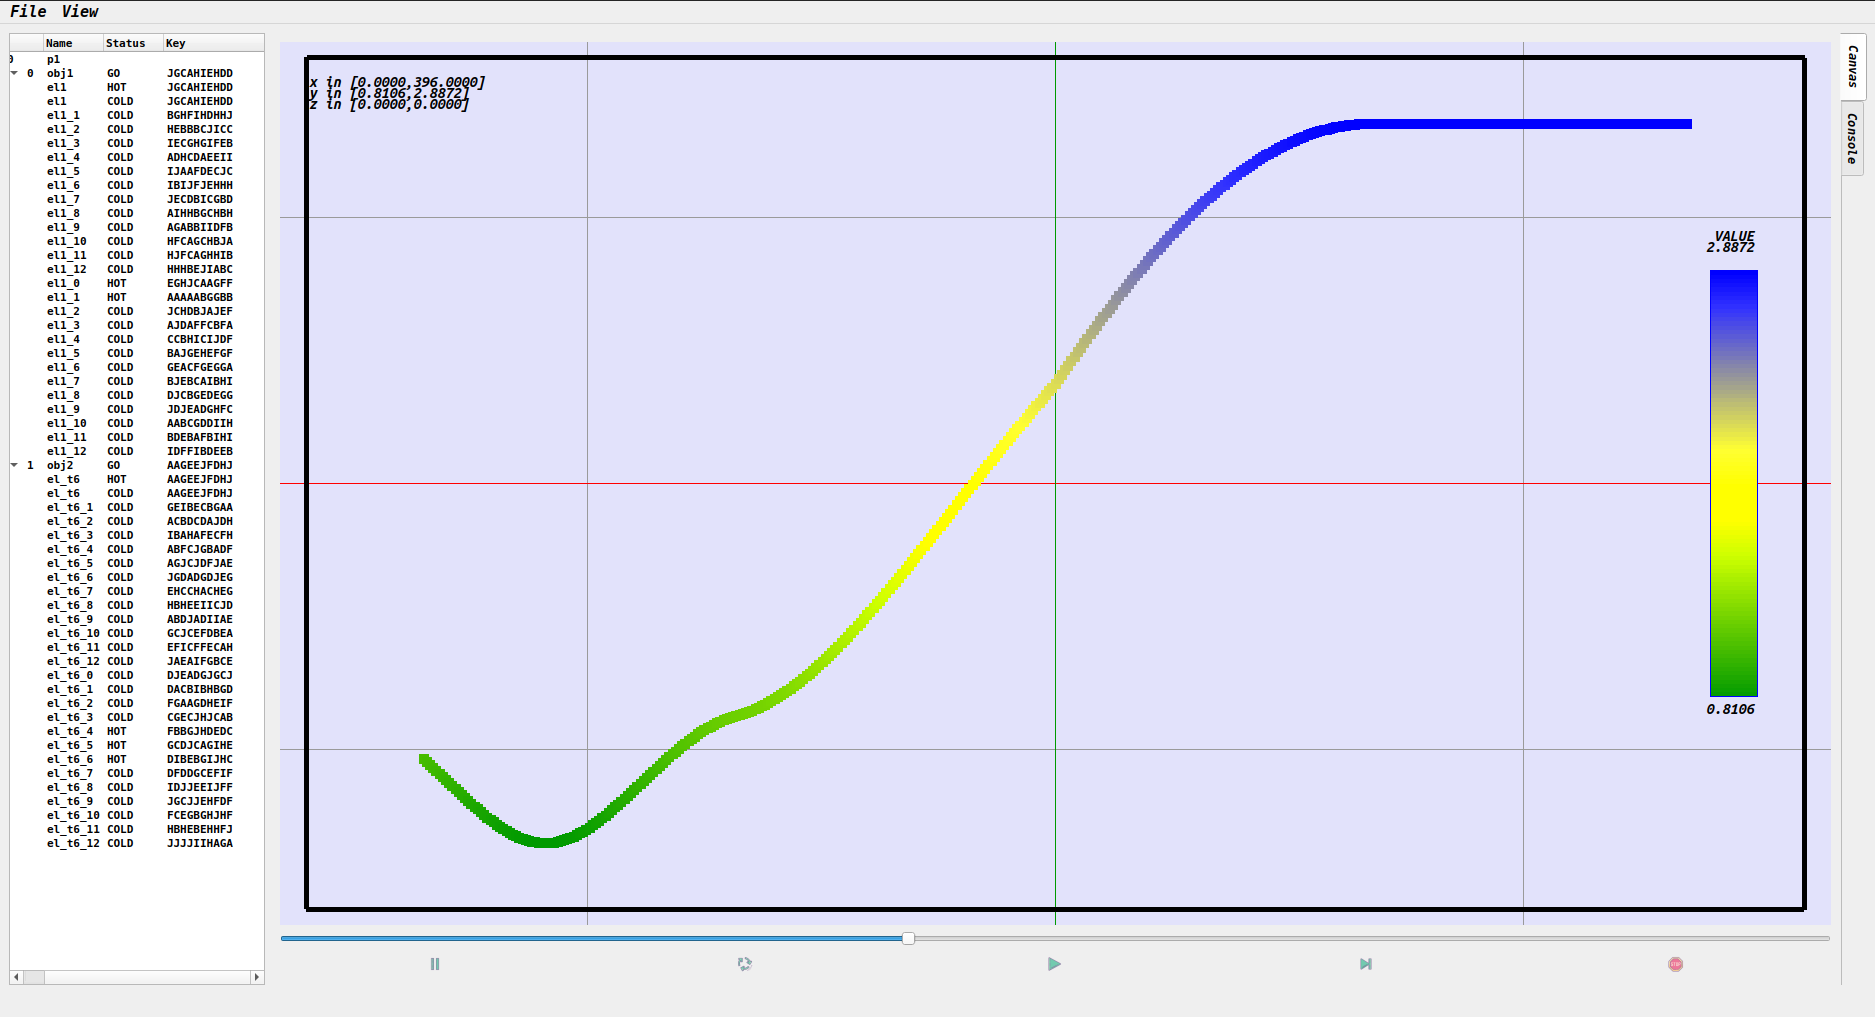
\includegraphics[width=.9\linewidth]{Figures/IGU_017.png}
	\caption{Mudanças gráficas observadas na Área de Trabalho ao trocar a aba selecionada, exibindo o elemento gráfico \textit{Canvas} com a aba \textit{Canvas} selecionada.}
	\label{fig:sfig1}
\end{figure}

\begin{figure}
	\centering
	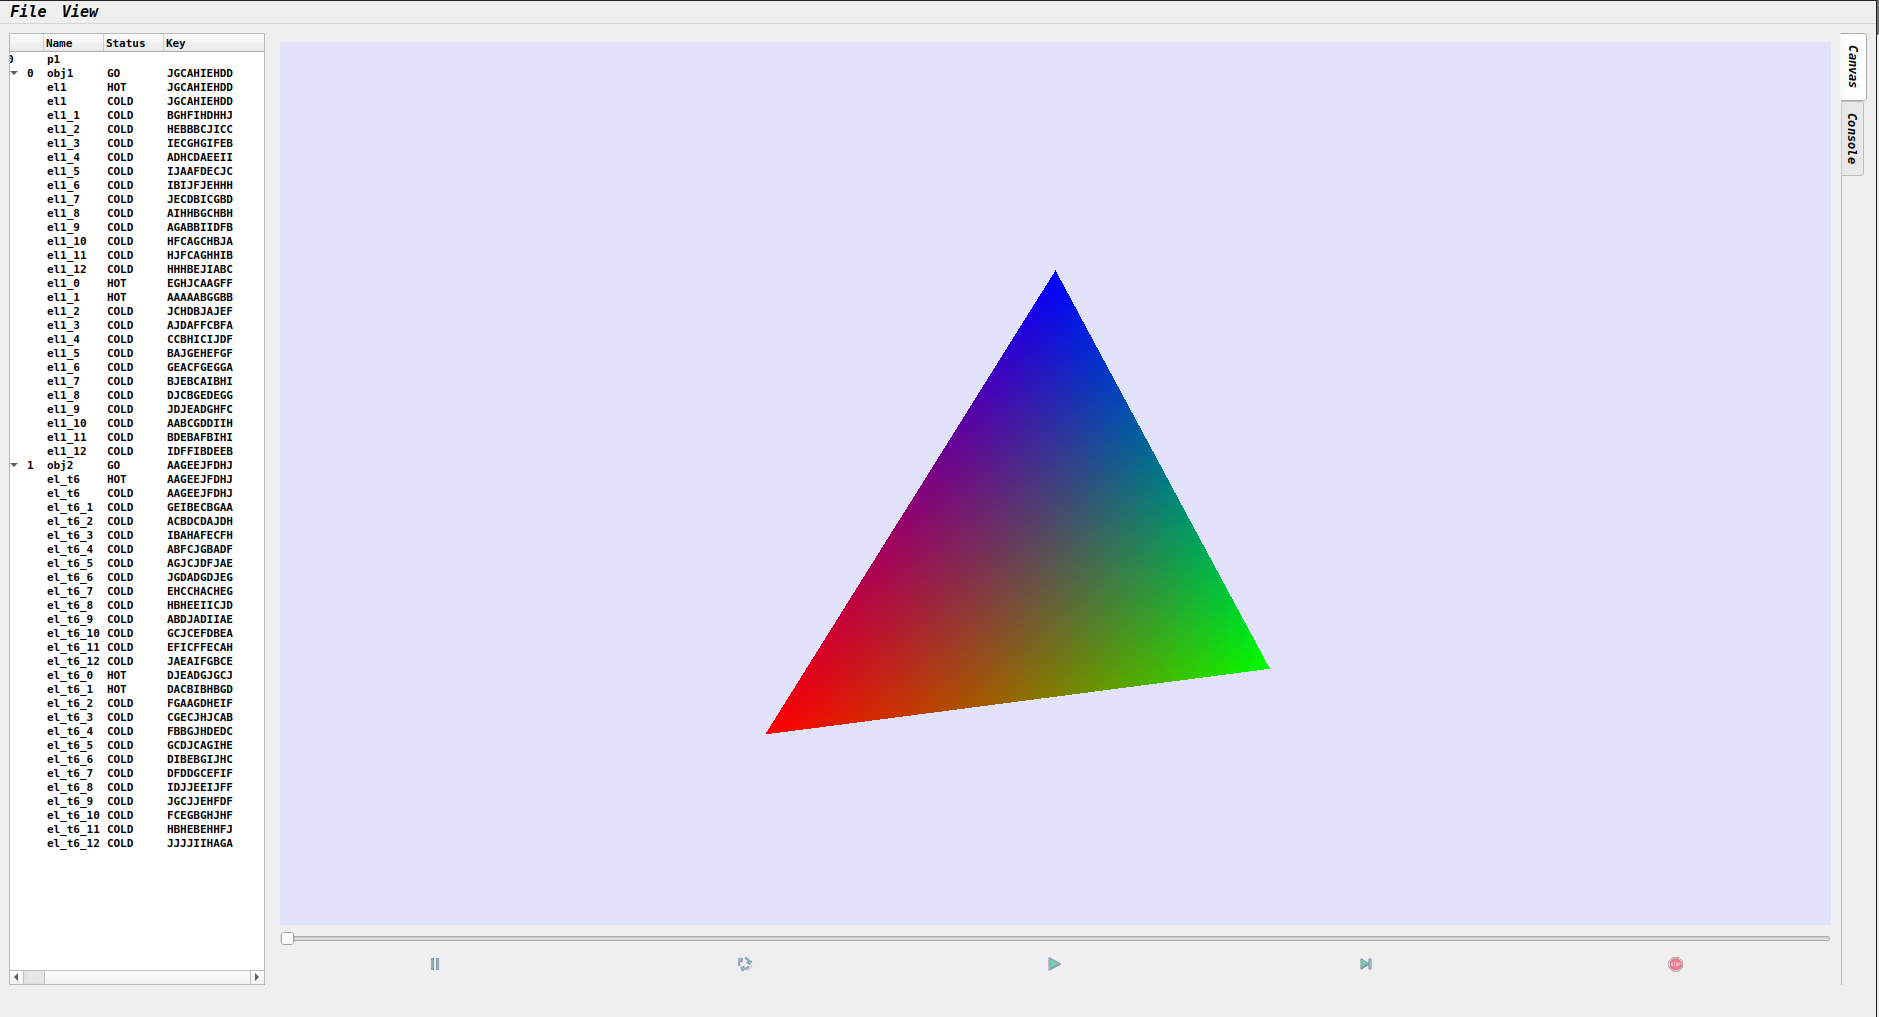
\includegraphics[width=.9\linewidth]{Figures/IGU_001.png}
	\caption{Mudanças gráficas observadas na Área de Trabalho ao trocar a aba selecionada, exibindo o elemento gráfico \textit{Console} com a aba \textit{Console} selecionada.}
	\label{fig:sfig2}
\end{figure}

A Figura~\ref{fig:fig} mostra as áreas de trabalho disponibilizadas ao selecionar uma das abas. Através da opção \textit{Canvas}, o elemento gráfico que contém um \textit{QWidget} cuja principal função é uma tela \textit{OpenGL}. Os objetos gráficos, resultados de iterações podem ser visualizados aqui. O funcionamento desta área de trabalho é descrito pela janela \textit{Canvas} e funciona como um 
reprodutor de vídeo.

As abas foram construídas para realizar todas as funções da ferramenta computacional com seus elementos gráficos. O ciclo de vida da thread \textit{WiseThreadPool} esta diretamente ligado À interface gráfica. Ao utilizar a interface gráfica para percorrer os elementos gráficos, ou executar a animação, irão desencadear chamadas diretas as threads disponibilizadas.

%--------------------------------------------------------------------------------%
\section{ÁRVORE DE PROJETOS}\label{sec:arvore_projetos}

Além da área de trabalho, o elemento gráfico que exibe a árvore de projetos se permanece fixa. Este elemento gráfico é um explorador de árvore \textit{QTreeWidget} que exibe todos os projetos carregados e suas estruturas. Esta árvore permite rapidamente verificar os elementos criados, seus nomes, suas chaves únicas e seu status atual.

\begin{figure}[!htbp]
	\centering
	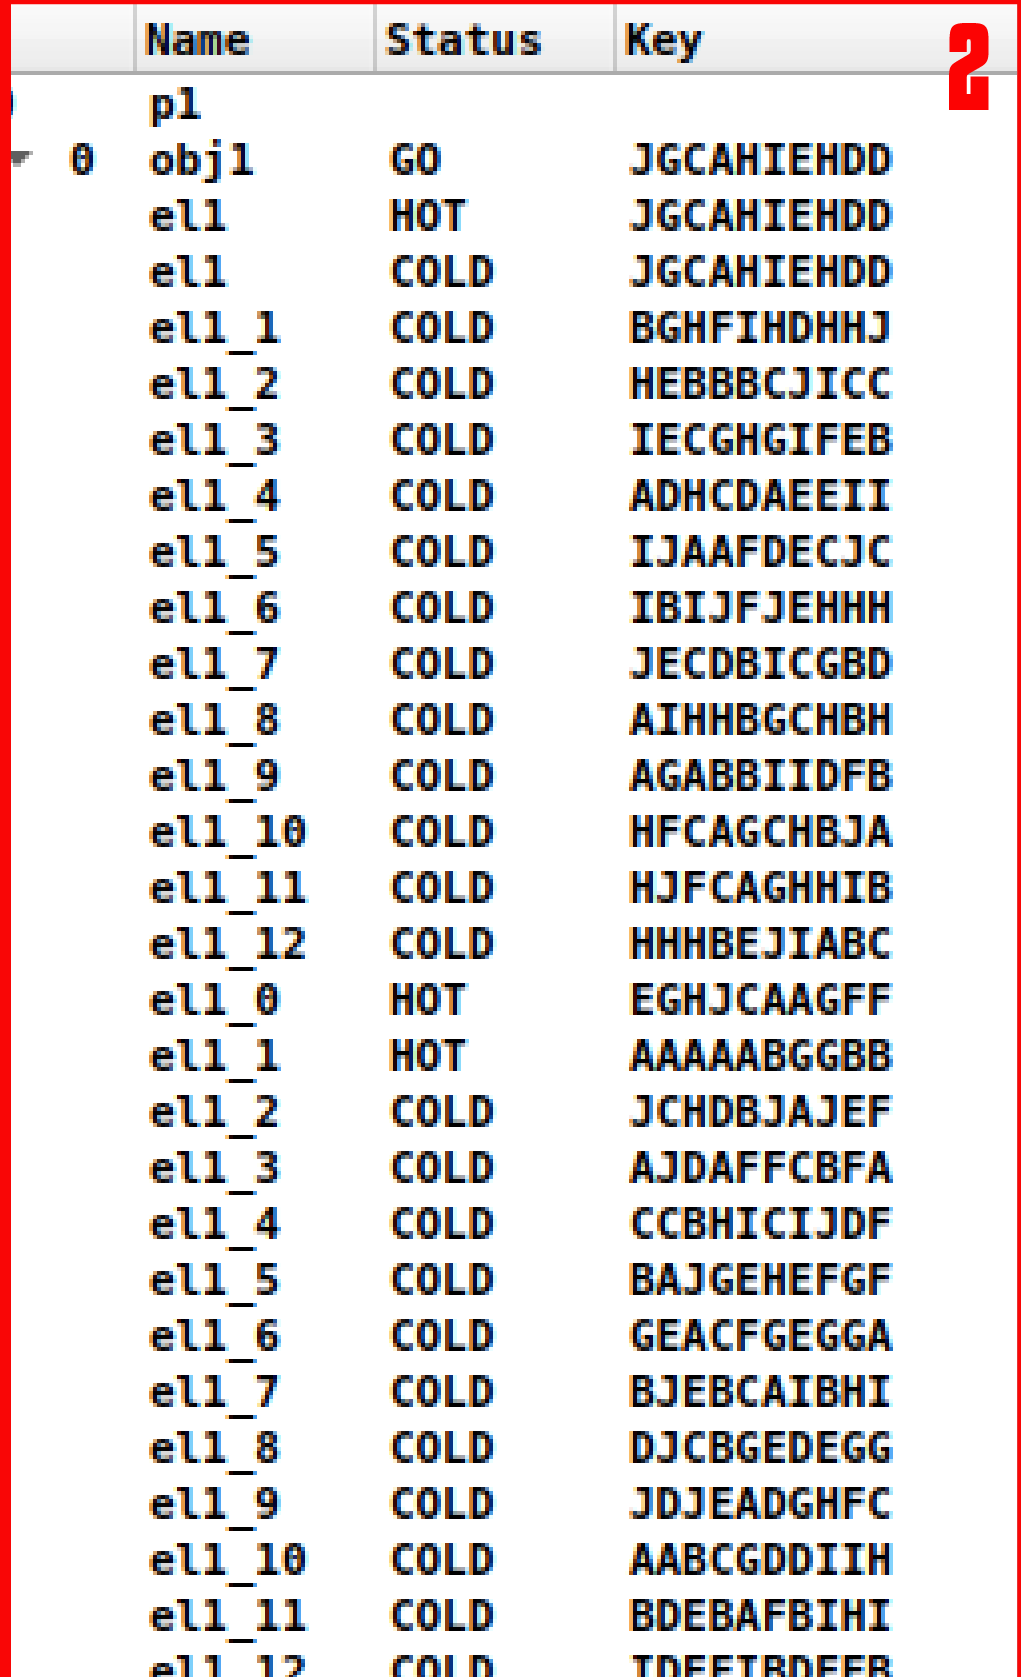
\includegraphics[width=0.4\linewidth]{Figures/IGU_001c.png}
	\caption{Árvore de projetos, na imagem a ferramenta apresenta um projeto inteligente $p1$, um objeto inteligente $obj1$ e seus elementos gráficos e inteligentes.}
	\label{fig:arvores}
\end{figure}

A Figura~\ref{fig:arvores} apresenta o elemento gráfico de uma árvore de projetos com objetos carregados. Na imagem está um projeto nomeado \textit{p1}, um objeto inteligente \textit{obj1} e diversos elementos inteligentes e gráficos. Como visto anteriormente quando o objeto está no estado \textit{GO} significa que ele já foi corretamente configurado e iterado. Dentro deste objeto inteligente estão os elementos inteligentes e gráficos. O primeiro elemento \textit{el1} é o elemento contido na estrutura \textit{Forno} e é o único elemento inteligente no estado \textit{Hot}. Em seguida estão os elementos inteligentes da estrutura \textit{Freezer}, seguidos pelos objetos gráficos.

Através da árvore de projetos é possível observar a troca de estado dos elementos, por exemplo, ao executar a animação os elementos gráficos serão sucessivamente aquecidos. Se observa que a mesma quantidade de elementos gráficos e inteligentes, mantendo a consistência do objeto inteligente, cada passo iterativo com sua respectiva representação gráfica.

%--------------------------------------------------------------------------------%
\section{JANELAS}\label{sec:janelas}

Nesta seção as janelas disponíveis no menu, descrito na Seção~\ref{sec:menu}, são exibidas e seu funcionamento descrito. Existem dois tipos de janelas disponibilizadas pela ferramenta computacional: \textit{Canvas}, que funciona como um reprodutor de vídeo, exibindo elementos gráficos sucessivamente; \textit{Jobs}, exibe todas as demandas criadas pelo programa enviadas à thread inteligente \textit{WiseThreadTool}. Esta última janela pode ser intstanciada apenas uma vez, enquanto diversos \textit{Canvas} podem ser disponibilizados e exibir diferentes objetos.

%--------------------------------------------------------------------------------%
\subsection{JANELA CANVAS}\label{sec:janela_canvas}

A janela e área de trabalho \textit{Canvas} possibilita que o usuário selecione o quadro à ser exibido. Cada quadro representa um objeto do tipo \textit{GraphicObject} que é um componente do modelo gráfico \textit{GraphicModel}. O quadro é selecionado através de uma barra de progresso, além de botões que alteram a animação feita com o objeto gráfico. Estes botões são:

\begin{itemize}
	\item \textbf{Pause}: Pausa a animação do objeto gráfico.
	\item \textbf{Repeat}: Este botão tem um funcionamento liga e desliga, ao ser ligado, quando a animação chegar ao último elemento gráfico retornará ao primeiro.
	\item \textbf{Play}:Este botão também tem um funcionamento liga e desliga, ao ser ligado, o elemento gráfico irá percorrer por todos os quadros da animação.
	\item \textbf{Avançar quadro}: Avança um quadro da animação.
	\item \textbf{Stop}: Caso o \textit{Play} esteja ativo ele é desativado e a tela volta ao primeiro elemento gráfico da animação.
\end{itemize}

Todas as funções do \textit{Canvas} só são disponibilizadas ao usuário depois que um objeto gráfico é ligado à tela \textit{OpenGl}. Neste cenário, quando cada quadro é selecionado é alterado quais objetos gráficos \textit{GraphicObject} estarão no estado aquecido \textit{Hot}. Isto foi feito utilizando a conexão entre objetos \textit{QObjects} e os elementos gráficos \textit{QWidget},desta forma a tela é capaz de acionar diretamente a estrutura do \textit{WiseThreadPool} e selecionar quais elementos debem ser aquecidos e exibidos. A mesma conexão é responsável por enviar a linha de comando da aba \textit{Console} à \textit{WiseThreadPool} para que seja executada e em seguida enviar a mensagem de resposta ao elemento textual.

\begin{figure}[!htbp]
	\centering
	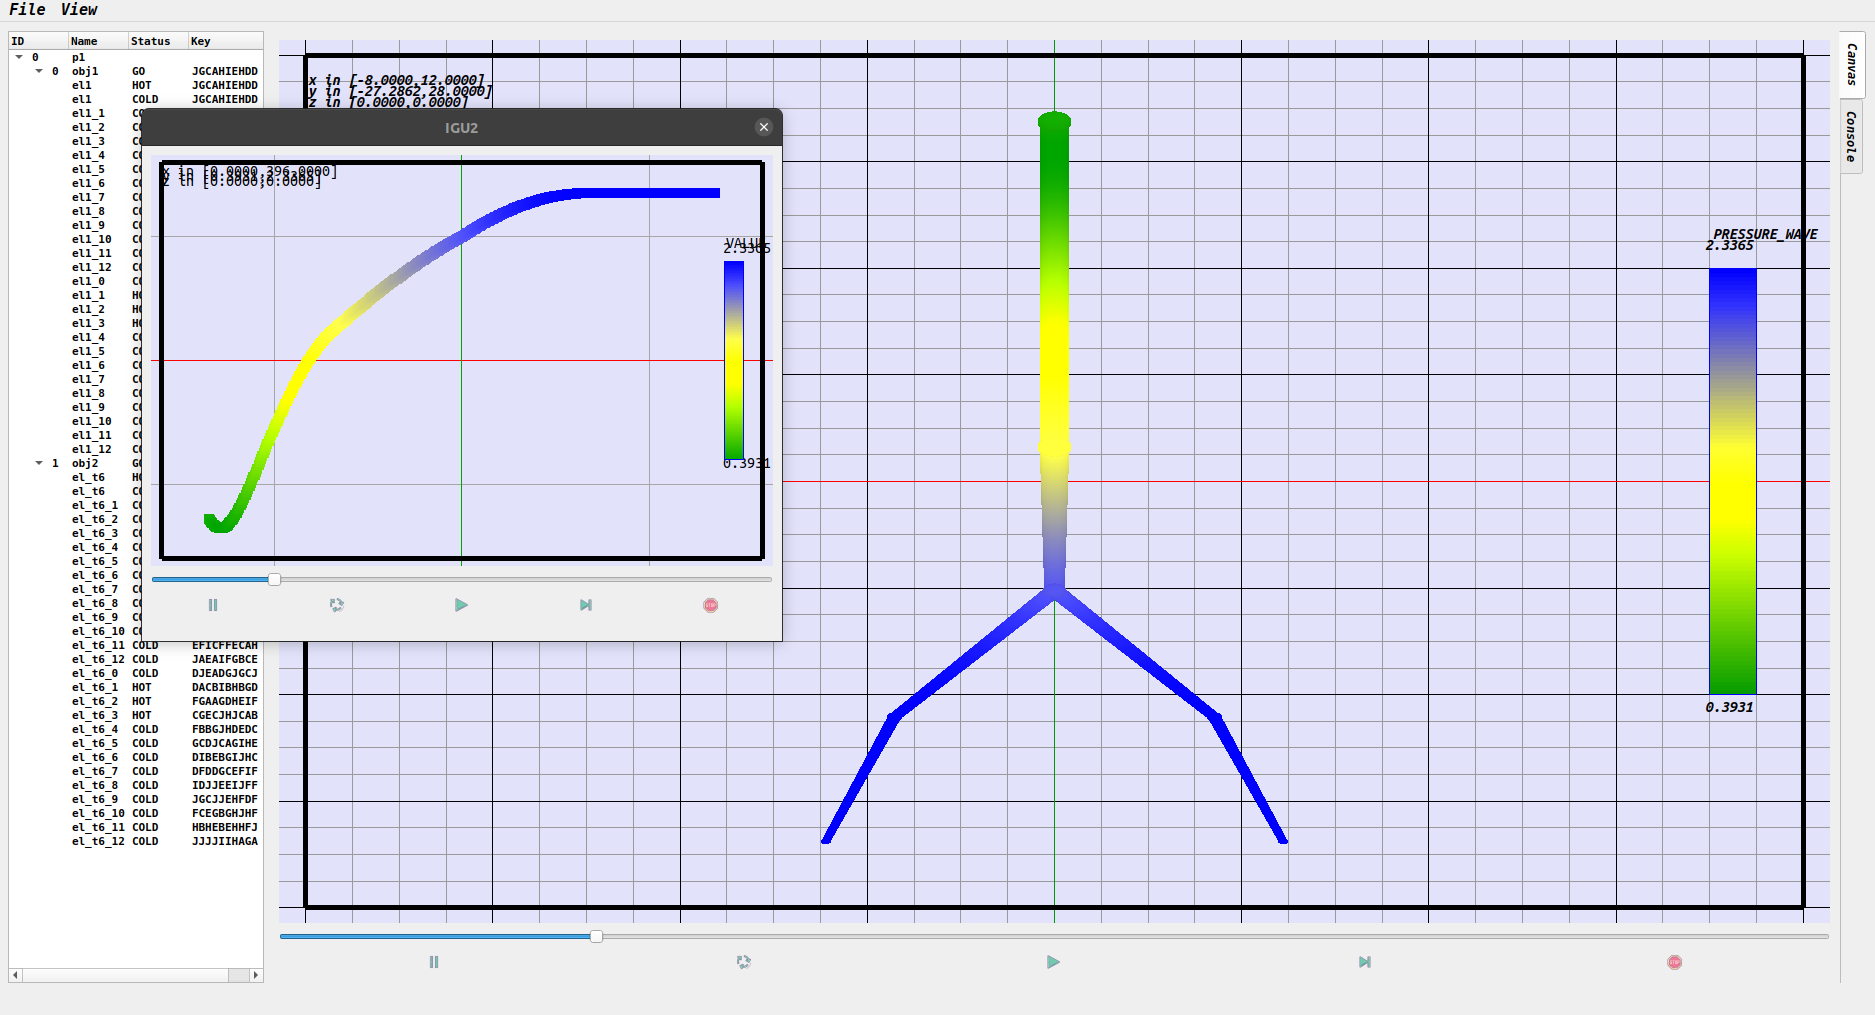
\includegraphics[width=\linewidth]{Figures/IGU_025.png}
	\caption{Janela \textit{Canvas} exibida sobre a área de trabalho \textit{Canvas}, a janela exibindo um gráfico obtido como resultado e a área de trabalho exibindo a árvore arterial estudada.}
	\label{fig:canvas}
\end{figure}

Durante sua execução esta janela irá selecionar o elemento gráfico \textit{GraphicElement} que deve ser exibido, selecionando o elemento através do objeto gráfico \textit{GraphicObject}. Para que o elemento seja exibido corretamente ele precisa estar no estado \textit{Hot}, que representa o momento em que o elemento está corretamente carregado em memória com o modelo geométrico e o parâmetro à ser exibido. Portanto, ao selecionar o elemento à ser exibido o \textit{Canvas} irá criar trabalhos de aquecimento de elementos. A coleção de objetos gráficos \textit{GraphicModel} é encarregada de enviar estes trabalhos a thread inteligente \textit{WiseThreadPool}.

%--------------------------------------------------------------------------------%
\subsection{JANELA JOBS}\label{sec:janela_jobs}

A janela \textit{Jobs} exibe uma listagem compreensiva dos processos inciados e enviados à thread inteligente \textit{WiseThreadPool}, cada comando executado via \textit{Console} ou elemento de interface gráfica irá gerar processos listados nesta janela.

\begin{figure}[!htbp]
	\centering
	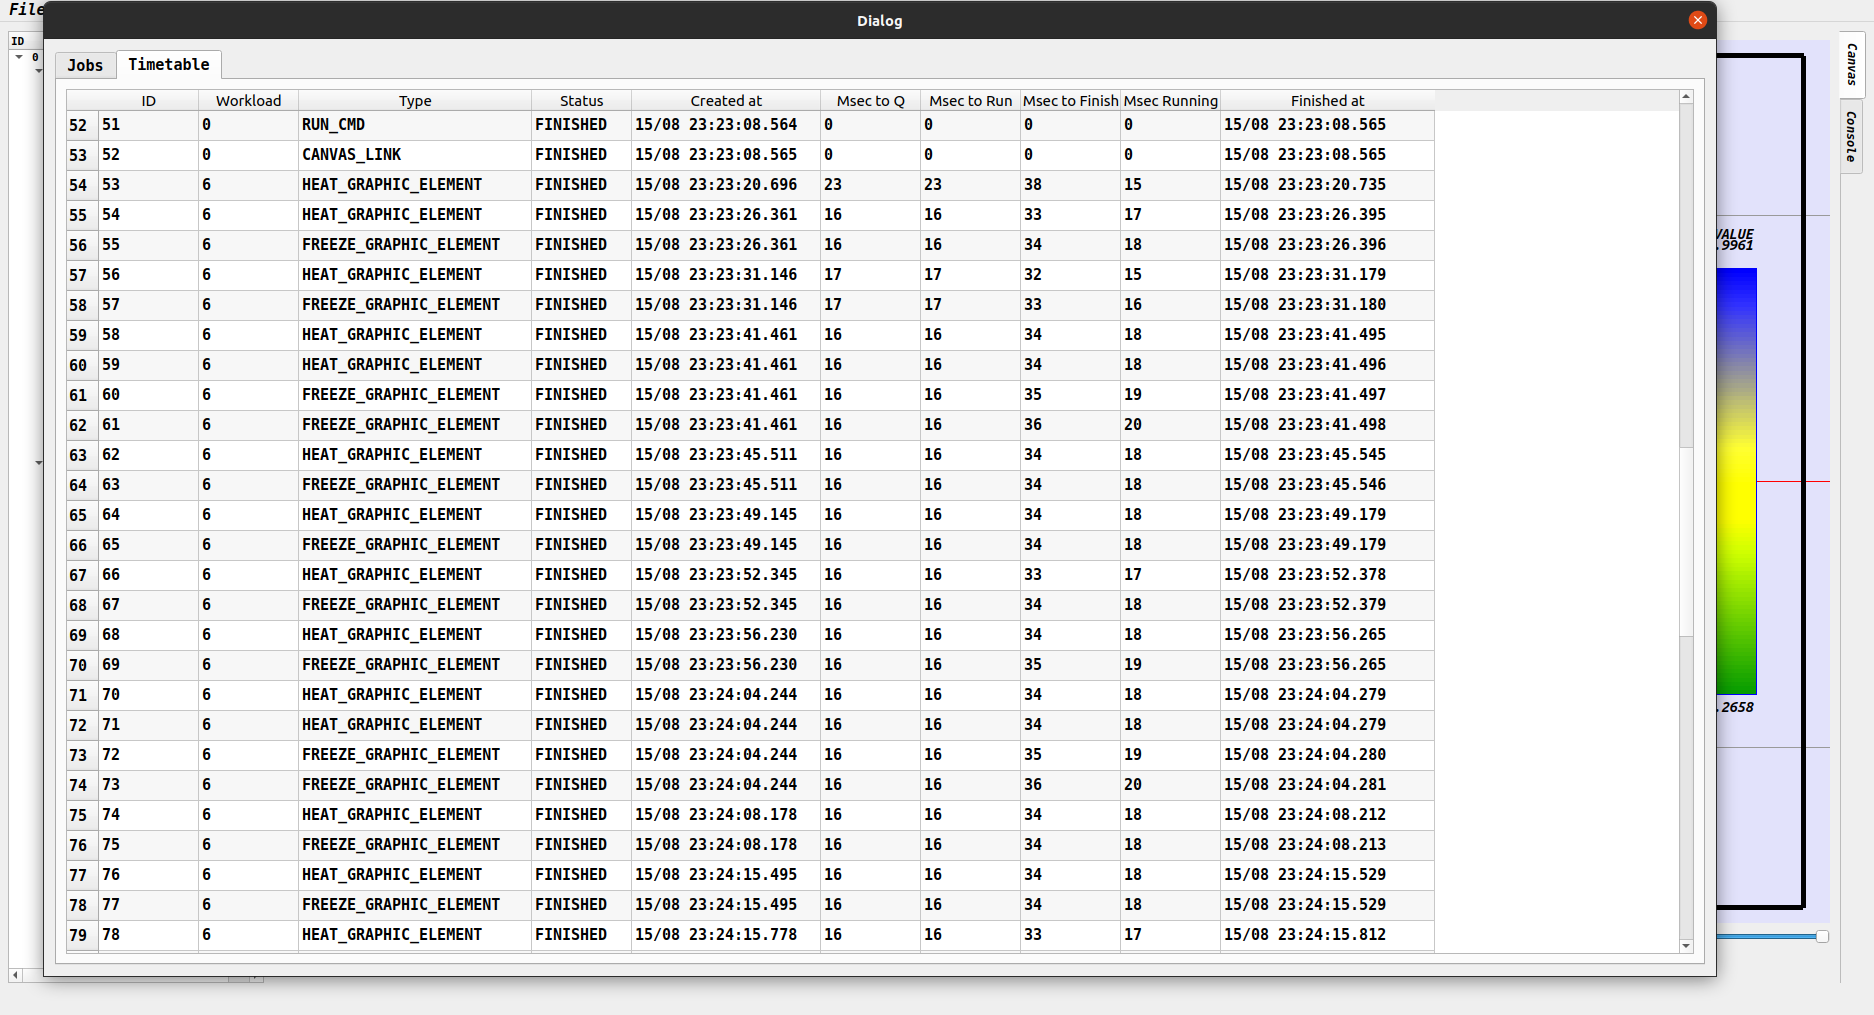
\includegraphics[width=\linewidth]{Figures/IGU_023.png}
	\caption{Janela \textit{Jobs} exibida com a aba \textit{Timetable} selecionada, a janela lista os trabalhos recebidos pela estrutura \textit{WiseThreadPool} e seus tempos de execução.}
	\label{fig:jobs}
\end{figure}

A Figura~\ref{fig:jobs} demonstra a tabela obtida lista todos os trabalhos recebidos pela thread inteligente \textit{WiseThread} e suas propriedades. Cada linha nesta janela representa um \textit{WiseJob}, as colunas descrevem propriedades de cada trabalho:

\begin{itemize}
	\item \textbf{ID}: Número de identificação.
	\item \textbf{Workload}: Número da carga de trabalho.
	\item \textbf{Status}: Estado do trabalho.
	\item \textbf{Created at}: Data de criação.
	\item \textbf{Msec to Q}: Milisegundos do momento da criação até a chegada a fila.
	\item \textbf{Msec to Run}: Milisegundos do momento da criação até a alocação do trabalho em uma thread.
	\item \textbf{Msec to Finish}: Milisegundos do momento da criação até o final de sua execução.
	\item \textbf{Msec Running}: Milisegundos no estado \textit{RUNNING}.
	\item \textbf{Finished at}: Data de finalização.
\end{itemize}

\begin{figure}[!htbp]
	\centering
	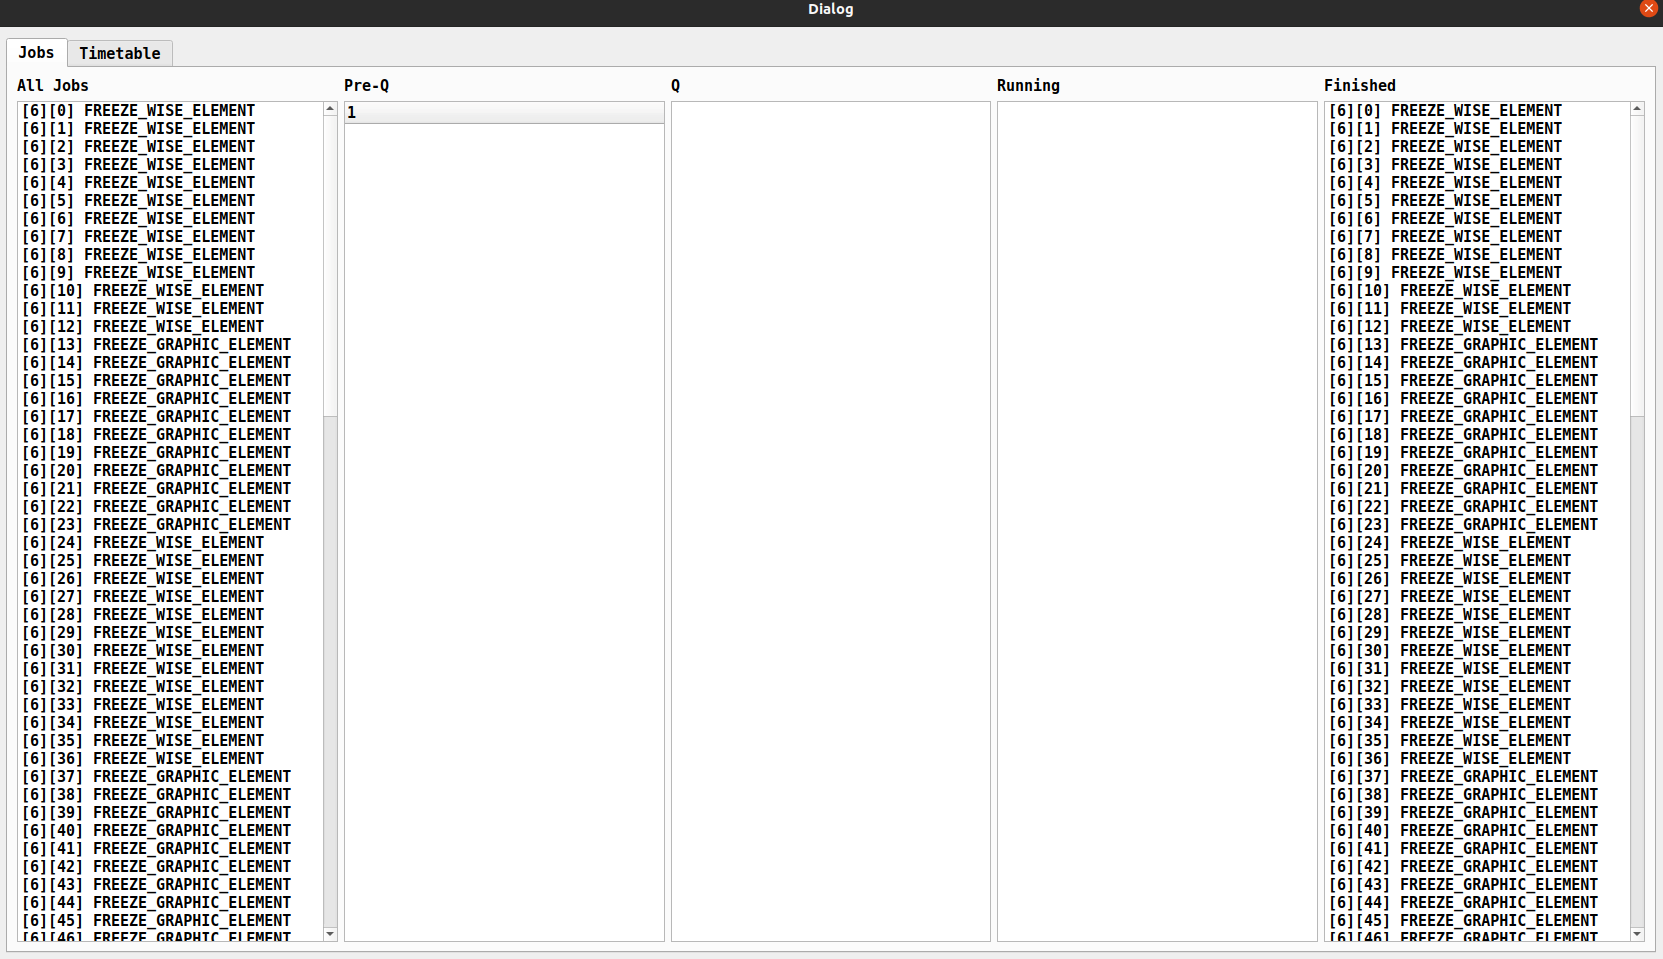
\includegraphics[width=\linewidth]{Figures/IGU_022.png}
	\caption{Janela \textit{Jobs} exibida com a aba \textit{Timetable} selecionada, a janela lista os trabalhos recebidos pela estrutura \textit{WiseThreadPool} e os separa logicamente pelas listas de espera.}
	\label{fig:jobs2}
\end{figure}

A Figura~\ref{fig:jobs2} demonstra as cinco listas exibidas ao selecionar a aba \textit{Timetable} da janela \textit{Jobs}. A primeira lista \textit{All Jobs} lista todos os trabalhos criados e as listas subsequentes listam as listas presentes no gerenciador de threads \textit{WiseThreadPool} descritas na Seção~\ref{sec:trabalhos}. Desta forma é possível verificar os trabalhos que aguardam execução, estão sendo executados e foram finalizados.